\documentclass[a4paper, 12pt]{article}
\usepackage{listings} 
\usepackage{xcolor}
\usepackage{mdframed}
\usepackage{graphicx}
\definecolor{code-gray}{gray}{0.93}
\begin{document}
\title{ECE 341 - Lab \#5}
\author{Collin Heist}
\date{\today}
\maketitle
\pagenumbering{roman}
\tableofcontents
\lstlistoflistings
\newpage
\pagenumbering{arabic}

\section{Introduction}
The purpose of this lab is to re-implement the previous lab, \textbf{Lab \#4}, but to use only foreground processes. I'll be using two interrupts for this current lab, one for Timer 1 (set to one millisecond), and the second for the button presses on \textbf{BTN1} and \textbf{BTN2}. Unlike the previous lab's, this code will not have multi or single-rate processes in the \textbf{main()} function, it will instead have all the processing code through the various Interrupt Service Routines.

The only relevant background information is the configuration of the interrupts. I'll add all the necessary interrupt configuration to the \textbf{system\_init()} function. After configuring both of these interrupts, they will both need their respective interrupt service routines (ISR's). These routines are called by the \textit{system}, and when the necessary interrupt condition is met (either one millisecond passing, or a button press) the ISR is then automatically run by the system. Because of the fact they're executed automatically by the micro-controller, my code will have no direct calls to the ISR functions. In fact, it is actually impossible to call an ISR directly (like a normal function).

The ISR's require special syntax because they require special parameters. In particular, you need to tell the compiler which interrupt vector to tie that particular ISR. This ties each interrupt, so either the button presses or timer, to the respective function execution (so that the right routine is called when a flag is triggered). In the unlikely event two interrupts are triggered at exactly the same time, or one interrupt is triggered during the execution of the another, the priority of those respective interrupts is what determines which takes precedence. Our processor, the \textbf{PIC 32} supports 7 levels of priority (plus priority 0 for the background tasks), which a higher level signifying a more important task.

For this lab, no code we'll be executing fits this priority, but if it is essential that a section of code is uninterrupted, interrupts can be temporarily disabled for the runtime of that code's execution. An example of this type of code would be timing-specific code, like responses to incoming signals and all that. Rather than giving that whole chunk of code a higher priority than the other interrupts, disabling and afterwards re-enabling interrupts allows for only the 'protected' bits to execute unimpeded. This type of protection can be implemented by disabling the interrupts with the \textbf{ INTDisableInterrupts()} function, and then once the protected code has been finished, re-enabling them with \textbf{INTEnableInterrupts()}. A possible consequence of this type of code is that very high-priority interrupt routines might be addressed later than you'd like, because their code could not be executed until the interrupts were re-enabled. To apply this example to the lab, if we protected the motor output code (for example), but then the one millisecond Timer 1 interrupt triggered during that block of code, the delay would be off by however long it took to execute that chunk of code.

\section{Implementation}
The first thing that I needed to change was the \textbf{system\_init()} function. In previous labs, we just needed to initialize the Cerebot, and then set the buttons and pins as inputs and outputs. The adjustments I've made are attached:

	\begin{mdframed}[backgroundcolor=code-gray, roundcorner=10pt,
								innerleftmargin=5, innertopmargin=5, innerbottommargin=5]	
	\begin{lstlisting}[language=C, caption=System Initialization, tabsize=2]
	void system_init(void) {
		... // I/O Config. from Lab #4

		OpenTimer1(T1_ON | T1_SOURCE_INT
			| T1_PS_1_1, T1_TICK-1);
		mT1SetIntPriority(2);
		mT1SetIntSubPriority(0);
		mT1IntEnable(1);

		mCNOpen(CN_ON,(CN8_ENABLE | CN9_ENABLE), 0);
		mCNSetIntPriority(1);
		mCNSetIntSubPriority(0);
		unsigned int x = PORTReadBits(IOPORT_G,
			BTN1 | BTN2);
		mCNClearIntFlag();
		mCNIntEnable(1);

		INTEnableSystemMultiVectoredInt();
	}
	\end{lstlisting}
	\end{mdframed}
	
I did not include the unchanged code from the previous labs. The above code instead configures the two necessary interrupts for this lab. Timer 1 is opened with the necessary period of one millisecond (where \textbf{T1\_TICK-1} is defined in the header file). The timer's priority is then set in accordance with the lab worksheet, and finally it is enabled.

Afterwards, the change notice interrupt is setup in a similar way. Using the provided change notice table, we setup the interrupt for \textbf{CN8} and \textbf{CN9}, which correspond to \textbf{BTN2} and \textbf{BTN1}. The buttons are given a priority lower than the timer interrupt, and then turned on, finishing the system initialization.

With both interrupts configured, the next bit of code that needed to be written was their respective interrupt service routines (\textit{ISR)}. The ISR for Timer 1 is shown below:

	\begin{mdframed}[backgroundcolor=code-gray, roundcorner=10pt,
								innerleftmargin=5, innertopmargin=5, innerbottommargin=5]	
	\begin{lstlisting}[language=C, caption=Timer 1 Interrupt Service Routine, tabsize=2]
	void __ISR(_TIMER_1_VECTOR, IPL2) Timer1Handler() {
		LATBINV = LEDA;
		if (!(--step_delay)) {
			stepper_state_machine();
			unsigned int del = (control_mode & 12) >> 2;
			unsigned int rev_min  = (del == RPM10) ?
				10 : (del == RPM15) ? 15 : 25;
			step_delay = 1.0 /
				((float) rev_min * 100.0 / 60.0 / 1000.0);
		}
		mT1ClearIntFlag();
	}
	\end{lstlisting}
	\end{mdframed}
	
This code is largely identical to the previous week's \textbf{step\_delay} if statement, and it is functionally equivalent. The function is first declared as an ISR, hence the abnormal syntax, and then the step delay is checked. As opposed to previous labs, where the current value of step delay was passed \textit{into} a function and then decremented, since an ISR cannot have any parameters passed into it (by reference or by value), \textbf{step\_delay} is a \textit{global} variable so it can be changed anywhere. If the delay is at zero (meaning the proper time has passed), then state machine is progressed, and then the \textbf{step\_delay} is reset to the proper value based on the current value of \textbf{control\_mode} (another global variable). Independent of whether or not a step was taken, the interrupt flag is finally cleared to prevent the ISR from constantly triggering.

Just like how the first ISR follows the same general structure as the \textbf{step\_delay} if statement from the previous Lab, the button ISR mirrors the \textbf{button\_delay} statement from that same lab. That's shown in Listing 3:
\newpage
	\begin{mdframed}[backgroundcolor=code-gray, roundcorner=10pt,
								innerleftmargin=5, innertopmargin=5, innerbottommargin=5]	
	\begin{lstlisting}[language=C, caption=Button Interrupt Service Routine, tabsize=2]
	void __ISR(_CHANGE_NOTICE_VECTOR, IPL1)
		CNIntHandler() {
		
		LATBINV = LEDC;
		hw_delay(20);
		unsigned int buttons = read_buttons();
		decode_buttons(buttons);
		LATBINV = LEDC;

		mCNClearIntFlag();
	}
	\end{lstlisting}
	\end{mdframed}
	
This simple ISR utilizes the hardware-assisted delay from Lab \#2 to wait 20 milliseconds for the buttons to 'debounce' and settle on a steady-state value. Once that time has passed, the buttons are read (same way as before), and their value is stored in the local variable \textbf{buttons}. The reason I did not use a global variable here is because it was unnecessary as no other functions need access to the status of the buttons themselves, only the corresponding control mode (which is updated inside \textbf{decode\_buttons()}). Once again, after all the 'logic' has finished, the interrupt flag is cleared to allow the code to resume it's normal operation.

I changed only one line of the \textbf{decode\_buttons()} function. Rather than \textit{returning} the control mode, since it's value is being used by other functions throughout the program, and is primarily called by an ISR, the control mode is instead stored into a global variable.

	\begin{mdframed}[backgroundcolor=code-gray, roundcorner=10pt,
								innerleftmargin=5, innertopmargin=5, innerbottommargin=5]	
	\begin{lstlisting}[language=C, caption=Button Decoding, tabsize=2]
	void decode_buttons(unsigned int portG_state) {
		unsigned int btns = portG_state >> 6;
		control_mode = (btns < 2 ? 4 + btns :
			((btns & 1) << 3) + btns); // Global variable
	}
	\end{lstlisting}
	\end{mdframed}
	
And one more very small change was made to the \textbf{stepper\_state\_machine()} function. Previously, it took in the control mode as a parameter, and returned the output code that was then sent to the stepper motor. Since the ISRs need to access these variables globally, there is no need for a return or parameter.

	\begin{mdframed}[backgroundcolor=code-gray, roundcorner=10pt,
								innerleftmargin=5, innertopmargin=5, innerbottommargin=5]	
	\begin{lstlisting}[language=C, caption=Revised Finite State Machine, tabsize=2]
	void stepper_state_machine(void) {
		... // Same FSM code as Lab #4
		output_to_stepper_motor(return_modes[state]);
	}
	\end{lstlisting}
	\end{mdframed}
	
As shown above, the code now directly calls the \textbf{output\_to\_stepper\_motor()} function, rather than returning the value. 

With all the above-shown functions changed to use global variables and interact with the ISR as needed, the while loop was the only thing that needed to be changed. Because the interrupts are triggered automatically by the system when their respective conditions are met, the main \textbf{while(1)} loop does not need to contain any code. All the function calls are handled by each interrupt routine, leaving the \textbf{main()} function looking like this:

	\begin{mdframed}[backgroundcolor=code-gray, roundcorner=10pt,
								innerleftmargin=5, innertopmargin=5, innerbottommargin=5]	
	\begin{lstlisting}[language=C, caption=Infinite Program Loop, tabsize=2]
	int main() {
		system_init();
	
		while (1) {}
	
		return 0;
	}
	\end{lstlisting}
	\end{mdframed}
	

	
\section{Testing and Verification}
All relevant oscilloscope screen captures are listed in the \textbf{Attachments} section. In each capture, $D_0$ is \textbf{LEDA}, toggled every one millisecond; $D_1$ is \textbf{LEDB} that is toggled every time an output is sent to the motor; and $D_2$ is \textbf{LEDC}, that is toggled at the beginning and end of the button-press \textbf{ISR}. As evident in the captures, $D_2$ triggers when I push the button, and thanks to the interrupt priority level's being configured correctly, $D_0$ does not miss a pulse during the runtime of that \textbf{ISR}. This is present in all the captures, and shows that the priority level of the Timer 1 \textbf{ISR} is \textit{greater} than that of the change notice button-presses. This is done intentionally to maintain accurate timing schemes throughout the runtime of the lab.

Because the Timer 1 \textbf{ISR} has the highest priority in our program, there is literally nothing that will prevent the \textbf{ISR} from triggering as soon as the flag is set. This results in the stepper motor \textit{technically} running more accurately in this lab, relative to before. In the previous lab, there would be instances where the motor's code would execute when the button code did not, or the other way around. This would result in the stepper motor code executing with small variations in the time between pulses, depending on whether or not the buttons were checked, if the button was pressed, etc. Having all the motor triggered through \textbf{ISR} results in nothing possibly interrupting the code when it needs to execute, increasing the consistency of the delay between pulses.

\section{Conclusion}
This lab served as an excellent introduction of foreground tasks (interrupts) and how they're useful in implementing various programs. Having already done this lab a few times, one using simple round-robin scheduling, and one using multi-rate processes, this seems (to me) to be the most efficient implementation. The advantage of this kind of real-time control system with interrupts is how all control happens nearly instantaneously. In our previous labs that utilized polling of the timer interrupt flag (rather than configuring an ISR), a significant portion of the processor's computation time was spent just waiting for a flag to trigger. Compare that to this lab where the system is 'free' to do whatever it wants (even though nothing happens in this particular lab), and the interrupts trigger events on their own, this is far more efficient and responsive. Despite the benefits of an interrupt-driven control system, they're not inherently better all the time. An example of this would be our button presses. Handling the button input ASAP is largely useless for this type of application, because the user's ability to delineate a 100 millisecond response time from a 1 millisecond response time is largely negligible. For this reason, the necessary overhead of the interrupt \textit{might} make simple polling a more accurate fit.

In general, interrupt-based control schemes require more overhead, but are far quicker to respond, and great for urgent event handling. On the other hand, polling schemes are very easy to implement with practically no overhead, and great for non-essential tasks, especially if they happen are a fixed rate.

In a polling-based system, the worst-case for response is how often the polling cycle is. For example, if the relevant flag is polled once every cycle, and that cycle takes 10 ms and the flag is set right after it was polled, then the system will take 10 ms to respond.

On the other hand, if an interrupt-based system is used then the system will at most take as long as all interrupts that have a higher priority (in the rare case that all of those interrupts were triggered at the same time), plus the time an interrupt takes to trigger (essentially negligible). In this lab, for example, the longest possible time it would take for the button-press interrupt to execute would be the length of the Timer 1 interrupt's (as it is high priority, and there is no protected code).

\section{Attachments}
As previously said, $D_0$ is \textbf{LEDA}, toggled every one millisecond; $D_1$ is \textbf{LEDB} that is toggled every time an output is sent to the motor; and $D_2$ is \textbf{LEDC}, that is toggled at the beginning and end of the button-press \textbf{ISR}

\begin{figure}[htb]
\centering
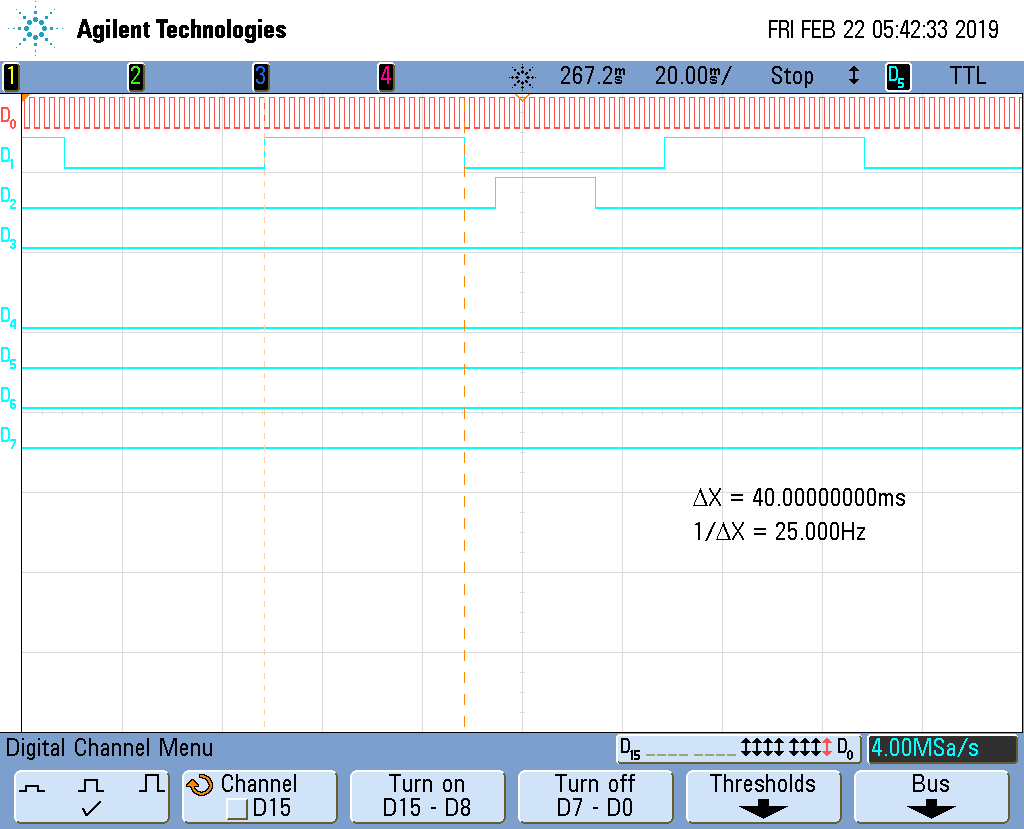
\includegraphics[width=.8\textwidth]{00.png}
\caption{The off-off, 40ms delay with button delay}
\end{figure}

\begin{figure}[htp]
\centering
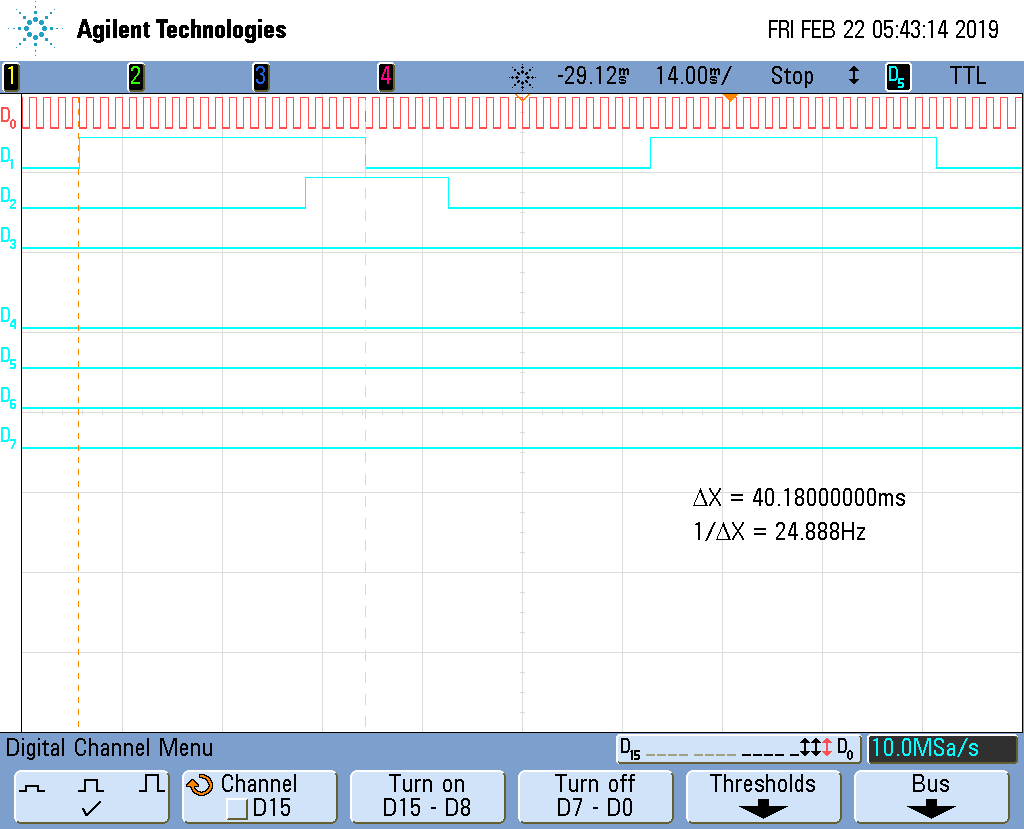
\includegraphics[width=.8\textwidth]{01.png}
\caption{The off-on 40ms delay}
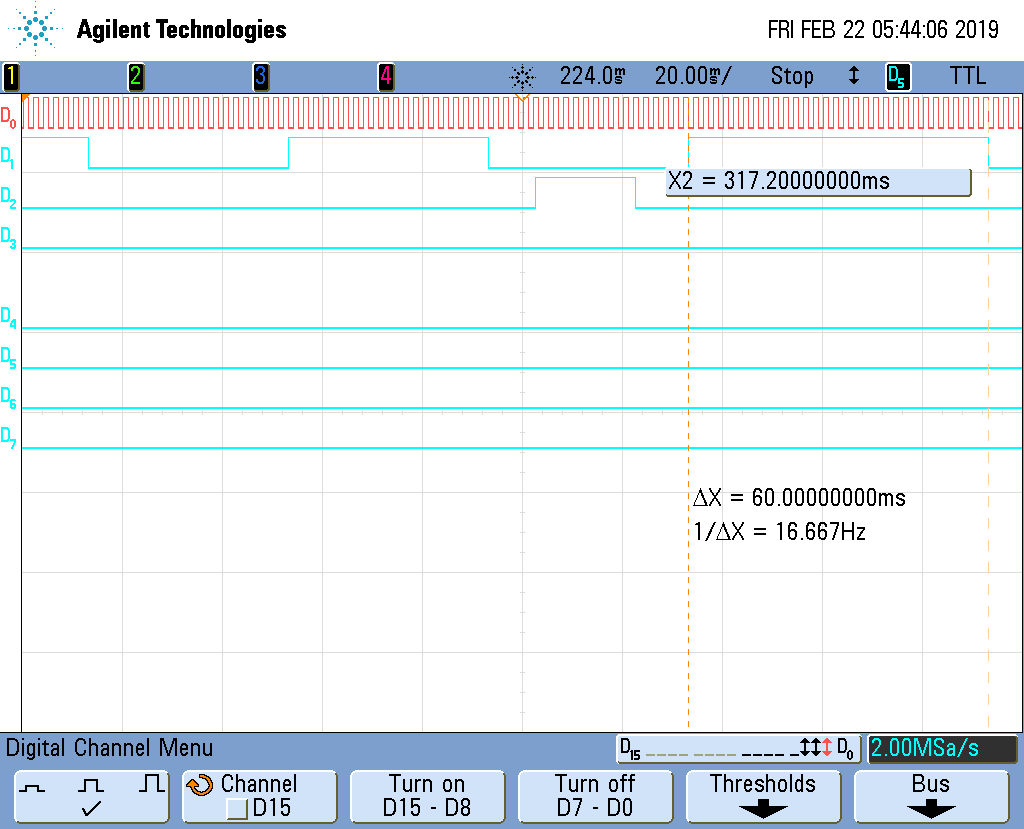
\includegraphics[width=.8\textwidth]{10.png}
\caption{The on-off 60ms delay}
\end{figure}

\begin{figure}[htb]
\centering
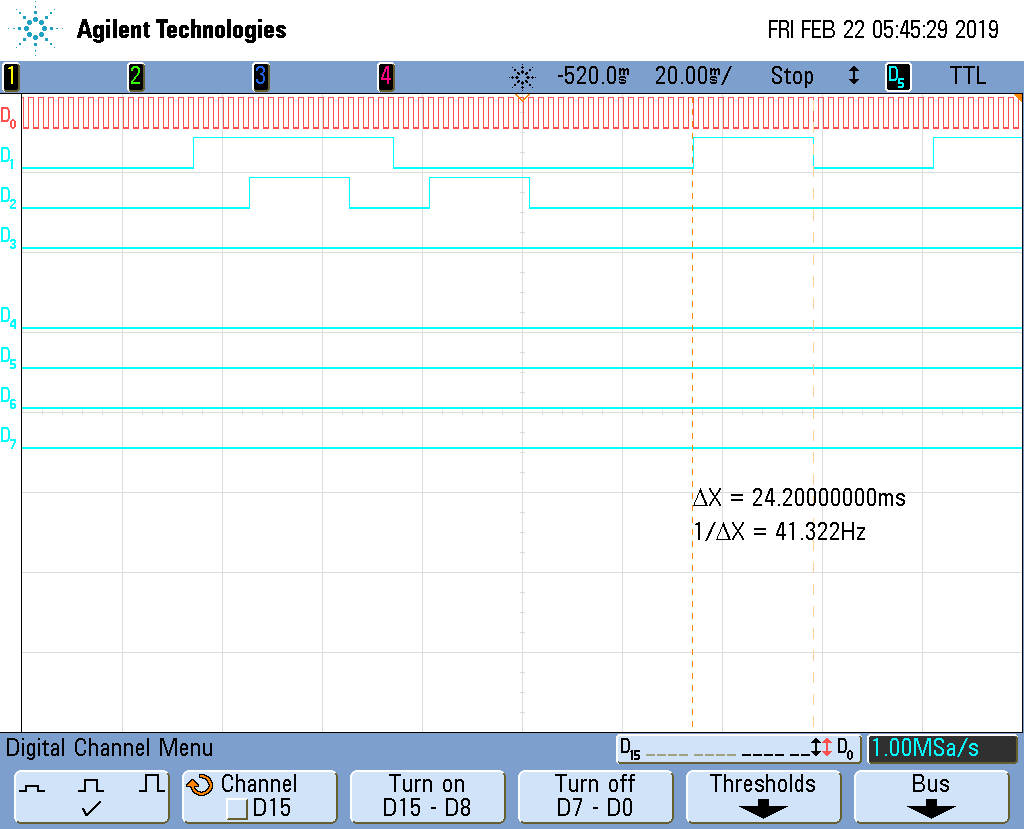
\includegraphics[width=.8\textwidth]{11.png}
\caption{The on-on 24ms delay}
\end{figure}

\end{document}